\section{Luồng ghi nhận câu hỏi chưa xử lý tốt}

Luồng này mô tả cơ chế hệ thống ghi lại các câu hỏi mà chatbot chưa xử lý tốt, bao gồm trường hợp không nhận diện được intent, trả lời chưa đúng trọng tâm hoặc phải rơi vào fallback nhiều lần. Đây là đầu vào rất quan trọng cho quy trình active training và cải thiện chất lượng hội thoại.

\begin{figure}[H]
    \centering
    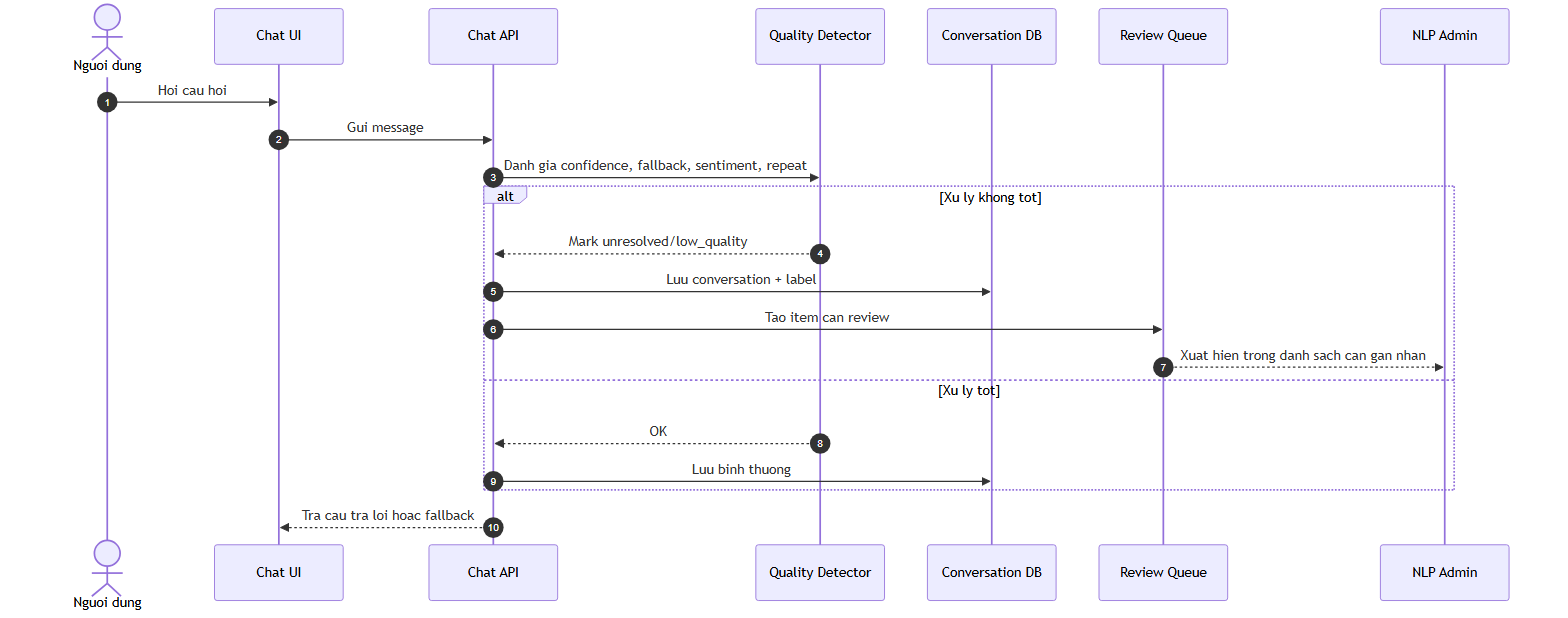
\includegraphics[width=\textwidth]{content/source/mermaid_sequence/seq_07.png}
    \caption{Luồng ghi nhận câu hỏi chưa xử lý tốt}
\end{figure}

Về mặt dữ liệu, sau khi một lượt hội thoại kết thúc hoặc bị đánh giá là chưa đạt, hệ thống tạo bản ghi chứa câu hỏi, ngữ cảnh liên quan, trạng thái xử lý và thông tin phản hồi của người dùng hoặc quản trị viên. Dữ liệu này được chuyển về khu vực quản trị để người vận hành xem xét, gán nhãn hoặc chuyển hóa thành ví dụ huấn luyện mới. Nhờ đó, các câu hỏi thực tế từ người dùng không bị thất thoát mà trở thành nguồn cải tiến hệ thống.
